


\tikzset{every picture/.style={line width=0.75pt}} %set default line width to 0.75pt        

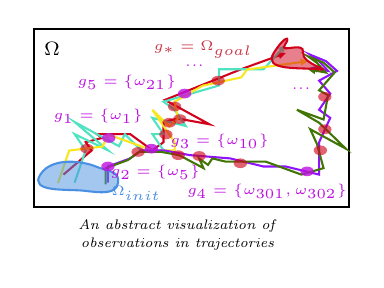
\begin{tikzpicture}[x=0.75pt,y=0.75pt,yscale=-1,xscale=1]
%uncomment if require: \path (0,1974); %set diagram left start at 0, and has height of 1974

%Shape: Rectangle [id:dp9996076613305621] 
\draw  [fill={rgb, 255:red, 255; green, 255; blue, 255 }  ,fill opacity=1 ] (24,1558.11) -- (176.1,1558.11) -- (176.1,1644) -- (24,1644) -- cycle ;
%Straight Lines [id:da05824332013205091] 
\draw [color={rgb, 255:red, 208; green, 2; blue, 27 }  ,draw opacity=1 ]   (142.67,1570.84) -- (124.28,1577.49) -- (87.26,1592.41) -- (108.68,1604.12) -- (93.53,1601.36) -- (86.58,1603.01) -- (86.58,1612.77) -- (82.05,1616.07) -- (81.22,1616.67) -- (78.65,1614.8) -- (70.51,1608.86) -- (54.44,1608.86) -- (57,1610.73) -- (49.09,1612.77) -- (51.85,1616.79) -- (38.38,1628.38) ;
\draw [shift={(145.49,1569.82)}, rotate = 160.12] [fill={rgb, 255:red, 208; green, 2; blue, 27 }  ,fill opacity=1 ][line width=0.08]  [draw opacity=0] (3.57,-1.72) -- (0,0) -- (3.57,1.72) -- cycle    ;
%Straight Lines [id:da9249559779542824] 
\draw [color={rgb, 255:red, 80; green, 227; blue, 194 }  ,draw opacity=1 ]   (143.47,1568.13) -- (134.78,1577.63) -- (113.36,1577.63) -- (113.36,1585.44) -- (86.58,1593.25) -- (91.93,1597.15) -- (97.29,1604.96) -- (81.22,1601.06) -- (86.58,1608.86) -- (81.22,1608.86) -- (86.58,1616.67) -- (75.87,1616.67) -- (67.94,1608.94) -- (65.16,1614.72) -- (43.73,1603.01) -- (59.8,1616.67) -- (43.73,1608.86) -- (49.09,1616.67) -- (43.73,1632.29) ;
\draw [shift={(145.49,1565.92)}, rotate = 132.45] [fill={rgb, 255:red, 80; green, 227; blue, 194 }  ,fill opacity=1 ][line width=0.08]  [draw opacity=0] (3.57,-1.72) -- (0,0) -- (3.57,1.72) -- cycle    ;
%Straight Lines [id:da17118391857757054] 
\draw [color={rgb, 255:red, 248; green, 231; blue, 28 }  ,draw opacity=1 ]   (153.23,1574.14) -- (126.83,1577.75) -- (124.07,1581.54) -- (105.41,1585.56) -- (91.93,1593.25) -- (93.53,1601.36) -- (89.34,1605.08) -- (81.22,1597.15) -- (91.93,1612.77) -- (91.93,1616.67) -- (81.22,1616.67) -- (59.99,1609.06) -- (57.21,1614.84) -- (41.14,1616.79) -- (35.78,1632.41) ;
\draw [shift={(156.2,1573.73)}, rotate = 172.2] [fill={rgb, 255:red, 248; green, 231; blue, 28 }  ,fill opacity=1 ][line width=0.08]  [draw opacity=0] (3.57,-1.72) -- (0,0) -- (3.57,1.72) -- cycle    ;
%Straight Lines [id:da6427777277243145] 
\draw [color={rgb, 255:red, 144; green, 19; blue, 254 }  ,draw opacity=1 ]   (160.23,1577.39) -- (165.84,1578.41) -- (161.56,1573.73) -- (157.27,1570.61) -- (164.86,1573.73) -- (170.13,1578.41) -- (161.56,1583.1) -- (166.91,1589.34) -- (161.56,1597.15) -- (166.91,1601.06) -- (161.56,1612.77) -- (161.56,1628.38) -- (145.49,1624.48) -- (134.78,1624.48) -- (128.99,1623.07) -- (125.92,1622.33) -- (121.57,1621.27) -- (118.71,1620.58) -- (107.96,1619.71) -- (99.43,1619.01) -- (95.23,1618.25) -- (86.58,1616.67) -- (75.87,1616.67) -- (70.51,1620.58) -- (59.8,1624.48) -- (59.8,1632.29) ;
\draw [shift={(157.27,1576.85)}, rotate = 10.33] [fill={rgb, 255:red, 144; green, 19; blue, 254 }  ,fill opacity=1 ][line width=0.08]  [draw opacity=0] (3.57,-1.72) -- (0,0) -- (3.57,1.72) -- cycle    ;
%Straight Lines [id:da7390021320622445] 
\draw [color={rgb, 255:red, 65; green, 117; blue, 5 }  ,draw opacity=1 ]   (159.15,1578.17) -- (164.77,1579.19) -- (160.49,1574.51) -- (156.2,1571.39) -- (163.79,1574.51) -- (169.06,1579.19) -- (161.56,1587.78) -- (165.84,1590.13) -- (163.7,1601.84) -- (150.85,1597.15) -- (161.56,1603.4) -- (174.41,1615.89) -- (157.27,1606.52) -- (160.49,1613.55) -- (163.7,1625.26) -- (152.99,1628.38) -- (135.85,1622.14) -- (123,1622.14) -- (116.57,1622.14) -- (110.14,1620.58) -- (108,1623.7) -- (103.72,1620.58) -- (105.86,1625.26) -- (94.16,1619.03) -- (85.51,1617.45) -- (74.8,1617.45) -- (69.44,1621.36) -- (58.73,1625.26) -- (58.73,1633.07) ;
\draw [shift={(156.2,1577.63)}, rotate = 10.33] [fill={rgb, 255:red, 65; green, 117; blue, 5 }  ,fill opacity=1 ][line width=0.08]  [draw opacity=0] (3.57,-1.72) -- (0,0) -- (3.57,1.72) -- cycle    ;
%Shape: Ellipse [id:dp30050508180239144] 
\draw  [draw opacity=0][fill={rgb, 255:red, 208; green, 2; blue, 27 }  ,fill opacity=0.62 ] (46.49,1615.89) .. controls (46.49,1614.6) and (47.93,1613.55) .. (49.71,1613.55) .. controls (51.48,1613.55) and (52.92,1614.6) .. (52.92,1615.89) .. controls (52.92,1617.19) and (51.48,1618.23) .. (49.71,1618.23) .. controls (47.93,1618.23) and (46.49,1617.19) .. (46.49,1615.89) -- cycle ;
%Shape: Ellipse [id:dp15311501498248647] 
\draw  [draw opacity=0][fill={rgb, 255:red, 208; green, 2; blue, 27 }  ,fill opacity=0.62 ] (90.49,1619.03) .. controls (90.49,1617.74) and (91.93,1616.69) .. (93.71,1616.69) .. controls (95.48,1616.69) and (96.92,1617.74) .. (96.92,1619.03) .. controls (96.92,1620.32) and (95.48,1621.37) .. (93.71,1621.37) .. controls (91.93,1621.37) and (90.49,1620.32) .. (90.49,1619.03) -- cycle ;
%Shape: Ellipse [id:dp19167487081496637] 
\draw  [draw opacity=0][fill={rgb, 255:red, 208; green, 2; blue, 27 }  ,fill opacity=0.62 ] (161.11,1606.52) .. controls (161.11,1605.23) and (162.54,1604.18) .. (164.32,1604.18) .. controls (166.09,1604.18) and (167.53,1605.23) .. (167.53,1606.52) .. controls (167.53,1607.82) and (166.09,1608.86) .. (164.32,1608.86) .. controls (162.54,1608.86) and (161.11,1607.82) .. (161.11,1606.52) -- cycle ;
%Shape: Ellipse [id:dp9201279867822619] 
\draw  [draw opacity=0][fill={rgb, 255:red, 208; green, 2; blue, 27 }  ,fill opacity=0.62 ] (120.4,1622.92) .. controls (120.4,1621.62) and (121.84,1620.58) .. (123.62,1620.58) .. controls (125.39,1620.58) and (126.83,1621.62) .. (126.83,1622.92) .. controls (126.83,1624.21) and (125.39,1625.26) .. (123.62,1625.26) .. controls (121.84,1625.26) and (120.4,1624.21) .. (120.4,1622.92) -- cycle ;
%Shape: Ellipse [id:dp3048334813609519] 
\draw  [draw opacity=0][fill={rgb, 255:red, 208; green, 2; blue, 27 }  ,fill opacity=0.62 ] (161.11,1590.91) .. controls (161.11,1589.61) and (162.54,1588.56) .. (164.32,1588.56) .. controls (166.09,1588.56) and (167.53,1589.61) .. (167.53,1590.91) .. controls (167.53,1592.2) and (166.09,1593.25) .. (164.32,1593.25) .. controls (162.54,1593.25) and (161.11,1592.2) .. (161.11,1590.91) -- cycle ;
%Shape: Ellipse [id:dp7290465976812913] 
\draw  [draw opacity=0][fill={rgb, 255:red, 208; green, 2; blue, 27 }  ,fill opacity=0.62 ] (86.13,1603.4) .. controls (86.13,1602.11) and (87.56,1601.06) .. (89.34,1601.06) .. controls (91.11,1601.06) and (92.55,1602.11) .. (92.55,1603.4) .. controls (92.55,1604.69) and (91.11,1605.74) .. (89.34,1605.74) .. controls (87.56,1605.74) and (86.13,1604.69) .. (86.13,1603.4) -- cycle ;
%Shape: Ellipse [id:dp6154487622646608] 
\draw  [draw opacity=0][fill={rgb, 255:red, 208; green, 2; blue, 27 }  ,fill opacity=0.62 ] (109.69,1583.1) .. controls (109.69,1581.8) and (111.13,1580.76) .. (112.9,1580.76) .. controls (114.68,1580.76) and (116.12,1581.8) .. (116.12,1583.1) .. controls (116.12,1584.39) and (114.68,1585.44) .. (112.9,1585.44) .. controls (111.13,1585.44) and (109.69,1584.39) .. (109.69,1583.1) -- cycle ;
%Shape: Ellipse [id:dp6108483574180856] 
\draw  [draw opacity=0][fill={rgb, 255:red, 189; green, 16; blue, 224 }  ,fill opacity=0.8 ] (77.56,1615.89) .. controls (77.56,1614.6) and (79,1613.55) .. (80.77,1613.55) .. controls (82.55,1613.55) and (83.98,1614.6) .. (83.98,1615.89) .. controls (83.98,1617.19) and (82.55,1618.23) .. (80.77,1618.23) .. controls (79,1618.23) and (77.56,1617.19) .. (77.56,1615.89) -- cycle ;
%Shape: Ellipse [id:dp08863924891219843] 
\draw  [draw opacity=0][fill={rgb, 255:red, 208; green, 2; blue, 27 }  ,fill opacity=0.62 ] (84.52,1609.06) .. controls (84.52,1607.77) and (85.96,1606.72) .. (87.73,1606.72) .. controls (89.51,1606.72) and (90.95,1607.77) .. (90.95,1609.06) .. controls (90.95,1610.35) and (89.51,1611.4) .. (87.73,1611.4) .. controls (85.96,1611.4) and (84.52,1610.35) .. (84.52,1609.06) -- cycle ;
%Shape: Ellipse [id:dp49807154634681794] 
\draw  [draw opacity=0][fill={rgb, 255:red, 208; green, 2; blue, 27 }  ,fill opacity=0.62 ] (91.21,1601.64) .. controls (91.21,1600.35) and (92.65,1599.3) .. (94.43,1599.3) .. controls (96.2,1599.3) and (97.64,1600.35) .. (97.64,1601.64) .. controls (97.64,1602.94) and (96.2,1603.98) .. (94.43,1603.98) .. controls (92.65,1603.98) and (91.21,1602.94) .. (91.21,1601.64) -- cycle ;
%Shape: Ellipse [id:dp17062416794692736] 
\draw  [draw opacity=0][fill={rgb, 255:red, 208; green, 2; blue, 27 }  ,fill opacity=0.62 ] (100.59,1619.41) .. controls (100.59,1618.11) and (102.03,1617.06) .. (103.8,1617.06) .. controls (105.57,1617.06) and (107.01,1618.11) .. (107.01,1619.41) .. controls (107.01,1620.7) and (105.57,1621.75) .. (103.8,1621.75) .. controls (102.03,1621.75) and (100.59,1620.7) .. (100.59,1619.41) -- cycle ;
%Shape: Ellipse [id:dp05427293190477478] 
\draw  [draw opacity=0][fill={rgb, 255:red, 189; green, 16; blue, 224 }  ,fill opacity=0.8 ] (152.54,1626.82) .. controls (152.54,1625.53) and (153.98,1624.48) .. (155.75,1624.48) .. controls (157.52,1624.48) and (158.96,1625.53) .. (158.96,1626.82) .. controls (158.96,1628.12) and (157.52,1629.16) .. (155.75,1629.16) .. controls (153.98,1629.16) and (152.54,1628.12) .. (152.54,1626.82) -- cycle ;
%Shape: Ellipse [id:dp0565658994925915] 
\draw  [draw opacity=0][fill={rgb, 255:red, 208; green, 2; blue, 27 }  ,fill opacity=0.62 ] (158.96,1616.67) .. controls (158.96,1615.38) and (160.4,1614.33) .. (162.18,1614.33) .. controls (163.95,1614.33) and (165.39,1615.38) .. (165.39,1616.67) .. controls (165.39,1617.97) and (163.95,1619.01) .. (162.18,1619.01) .. controls (160.4,1619.01) and (158.96,1617.97) .. (158.96,1616.67) -- cycle ;
%Shape: Ellipse [id:dp5007110255270828] 
\draw  [draw opacity=0][fill={rgb, 255:red, 189; green, 16; blue, 224 }  ,fill opacity=0.8 ] (57,1610.73) .. controls (57,1609.43) and (58.44,1608.38) .. (60.21,1608.38) .. controls (61.99,1608.38) and (63.43,1609.43) .. (63.43,1610.73) .. controls (63.43,1612.02) and (61.99,1613.07) .. (60.21,1613.07) .. controls (58.44,1613.07) and (57,1612.02) .. (57,1610.73) -- cycle ;
%Shape: Ellipse [id:dp22598728144573377] 
\draw  [draw opacity=0][fill={rgb, 255:red, 208; green, 2; blue, 27 }  ,fill opacity=0.62 ] (88.72,1595.59) .. controls (88.72,1594.3) and (90.16,1593.25) .. (91.93,1593.25) .. controls (93.71,1593.25) and (95.15,1594.3) .. (95.15,1595.59) .. controls (95.15,1596.88) and (93.71,1597.93) .. (91.93,1597.93) .. controls (90.16,1597.93) and (88.72,1596.88) .. (88.72,1595.59) -- cycle ;
%Shape: Ellipse [id:dp14749486568088088] 
\draw  [draw opacity=0][fill={rgb, 255:red, 189; green, 16; blue, 224 }  ,fill opacity=0.8 ] (93.54,1589.34) .. controls (93.54,1588.05) and (94.98,1587) .. (96.75,1587) .. controls (98.53,1587) and (99.97,1588.05) .. (99.97,1589.34) .. controls (99.97,1590.64) and (98.53,1591.69) .. (96.75,1591.69) .. controls (94.98,1591.69) and (93.54,1590.64) .. (93.54,1589.34) -- cycle ;
%Shape: Polygon Curved [id:ds6643267525526769] 
\draw  [color={rgb, 255:red, 74; green, 144; blue, 226 }  ,draw opacity=1 ][fill={rgb, 255:red, 74; green, 144; blue, 226 }  ,fill opacity=0.5 ] (27.21,1628.38) .. controls (30.38,1623.39) and (36.63,1621.99) .. (42.56,1622.18) .. controls (47.05,1622.33) and (51.36,1623.39) .. (53.99,1624.48) .. controls (60.1,1627.02) and (65.56,1626.63) .. (64.7,1632.29) .. controls (63.85,1637.95) and (56.88,1637.17) .. (48.64,1636.19) .. controls (40.39,1635.22) and (21.64,1637.17) .. (27.21,1628.38) -- cycle ;
%Shape: Polygon Curved [id:ds9461514343962948] 
\draw  [color={rgb, 255:red, 208; green, 2; blue, 27 }  ,draw opacity=1 ][fill={rgb, 255:red, 208; green, 2; blue, 27 }  ,fill opacity=0.5 ] (139.68,1569.82) .. controls (145.25,1561.04) and (148.01,1561.59) .. (145.04,1565.92) .. controls (142.07,1570.25) and (154.68,1563.87) .. (153.82,1569.53) .. controls (152.97,1575.19) and (169.35,1578.61) .. (161.11,1577.63) .. controls (152.86,1576.66) and (134.11,1578.61) .. (139.68,1569.82) -- cycle ;
%Shape: Ellipse [id:dp06406072166611776] 
\draw  [draw opacity=0][fill={rgb, 255:red, 208; green, 2; blue, 27 }  ,fill opacity=0.62 ] (71.13,1617.45) .. controls (71.13,1616.16) and (72.57,1615.11) .. (74.34,1615.11) .. controls (76.12,1615.11) and (77.56,1616.16) .. (77.56,1617.45) .. controls (77.56,1618.75) and (76.12,1619.8) .. (74.34,1619.8) .. controls (72.57,1619.8) and (71.13,1618.75) .. (71.13,1617.45) -- cycle ;
%Shape: Ellipse [id:dp049221150011381054] 
\draw  [draw opacity=0][fill={rgb, 255:red, 189; green, 16; blue, 224 }  ,fill opacity=0.8 ] (56.59,1624.48) .. controls (56.59,1623.19) and (58.03,1622.14) .. (59.8,1622.14) .. controls (61.58,1622.14) and (63.01,1623.19) .. (63.01,1624.48) .. controls (63.01,1625.77) and (61.58,1626.82) .. (59.8,1626.82) .. controls (58.03,1626.82) and (56.59,1625.77) .. (56.59,1624.48) -- cycle ;


% Text Node
\draw (68.95,1583.75) node  [font=\tiny,color={rgb, 255:red, 189; green, 16; blue, 224 }  ,opacity=1 ] [align=left] {$\displaystyle g_{5} =\{\omega _{21} \dotsc \}$};
% Text Node
\draw (82.63,1627.35) node  [font=\tiny,color={rgb, 255:red, 189; green, 16; blue, 224 }  ,opacity=1 ] [align=left] {$\displaystyle g_{2} =\{\omega _{5}\}$};
% Text Node
\draw (152.91,1586.86) node  [font=\tiny,color={rgb, 255:red, 189; green, 16; blue, 224 }  ,opacity=1 ] [align=left] {$\displaystyle ...$};
% Text Node
\draw (101.5,1575.93) node  [font=\tiny,color={rgb, 255:red, 189; green, 16; blue, 224 }  ,opacity=1 ] [align=left] {$\displaystyle ...$};
% Text Node
\draw (136.45,1636.35) node  [font=\tiny,color={rgb, 255:red, 189; green, 16; blue, 224 }  ,opacity=1 ] [align=left] {$\displaystyle g_{4} =\{\omega _{301} ,\omega _{302}\}$};
% Text Node
\draw (113.58,1612.35) node  [font=\tiny,color={rgb, 255:red, 189; green, 16; blue, 224 }  ,opacity=1 ] [align=left] {$\displaystyle g_{3} =\{\omega _{10}\}$};
% Text Node
\draw (55.11,1600.35) node  [font=\tiny,color={rgb, 255:red, 189; green, 16; blue, 224 }  ,opacity=1 ] [align=left] {$\displaystyle g_{1} =\{\omega _{1}\}$};
% Text Node
\draw (105.58,1568.35) node  [font=\tiny,color={rgb, 255:red, 202; green, 52; blue, 69 }  ,opacity=1 ] [align=left] {$\displaystyle g_{*} =\Omega _{goal}$};
% Text Node
\draw (73.43,1637.35) node  [font=\tiny,color={rgb, 255:red, 74; green, 144; blue, 226 }  ,opacity=1 ] [align=left] {$\displaystyle \Omega _{init}$};
% Text Node
\draw (32.91,1567.84) node  [font=\scriptsize] [align=left] {$\displaystyle \Omega $};
% Text Node
\draw (93.61,1653) node   [align=left] {{\tiny \textit{An abstract visualization of}}};
\draw (93.61,1662) node   [align=left] {{\tiny \textit{observations in trajectories}}};

\end{tikzpicture}